\tikzstyle{block} = [rectangle, draw, text width=9em, text centered, minimum height=4em]
\tikzstyle{line} = [-triangle 45, draw]


\chapter{Технологический раздел}
\section{Упрощение поиска ближайших частиц}
Для ускорения поиска соседних частиц активно применяется разбиение пространства \cite{harada}. В качестве простого и достаточно эффективного разбиения удобно взять разбиение трёхмерной сеткой.

Тогда индекс ячейки этой сетки для частицы $i$:
\[ \vect c(\vect r_i)=\left\lfloor\frac{\vect r_i-\vect r_c}{s}\right\rfloor,\]
\begin{conditions}
  $\vect r_c$ & координаты нулевой ячейки;\\
  $\vect r_i$ & координаты частицы $i$;\\
  $s$ & размер ячейки.
\end{conditions}

Стоит заметить, что в данной работе для симуляции задействована область $0..1$, а значит нулевая ячейка будет располагаться в памяти как первый элемент массива. Поэтому для упрощения расчётов выгодно положить $\vect r_c=-s$, что позволит избавиться от проверок выхода за пределы сетки.

Таким образом, итоговая формула для вычисления индекса ячейки принимает вид
\begin{equation} \label{eq:cell}
  \vect c(\vect r_i)=\bigg\lfloor\frac{\vect r_i}{s}\bigg\rfloor+1,
\end{equation}

Теперь, имея индекс ячейки, необходимо связать ячейку с данной частицей. Однако для экономии вычислительных ресурсов и памяти, было решено упростить физическую модель в пользу упрощения расчетов и хранить средние характеристики частиц для каждой ячейки вместо непосредственно самих частиц. Таким образом, для обхода соседних частиц, достаточно проанализировать <<усреднённые частицы>> в соседних ячейках.

Размер ячейки для для симуляции может быть вычислен как
\begin{equation}
  s(h, n) = \frac{2h}{n}
\end{equation}
\begin{conditions}
  $h$ & радиус сглаживания;\\
  $n$ & кол-во соседей по одной оси ($3, 5, ...$).
\end{conditions}

Размер же вокселя для триангуляции задаётся пользователем и напрямую влияет на качество получаемого изображения.


\section{Сглаживание воксельной сетки}
Качество результирующего изображения сильно зависит от размера воксельной сетки. Чем меньше размер вокселя, тем качество выше. Однако при уменьшении размера, количество частиц может не хватать для заполнения отдельных вокселей, что ведёт к образованию дыр и нерегулярности структуры.

Для решения данной проблемы применяется сглаживание сетки: для каждого вокселя применяется сглаживающее трёхмерное ядро, которое чаще всего является некоторой аппроксимацией гауссово ядра сглаживания.

В данной работе при сглаживании для каждого вокселя учитываются шесть прилегающих вокселей:
\begin{equation} \label{eq:spreading}
  p_i\gets \frac{1}{8}\left(2p_i+\sum_{j=0}^5p_j\right),
\end{equation}
\begin{conditions}
  $p_i$ & значение потенциала в текущем вокселе;\\
  $p_j$ & значение потенциала в вокселях, имеющих общую грань с данной.
\end{conditions}


\section{Описание алгоритма}
Исходя из проведённых в ходе работы исследований и полученных знаний, можно составить полный алгоритм моделирования поведения жидкости и её рендеринга.


\subsection{Симуляция}
Краткая схема работы алгоритма симуляции представлена на рис.~\ref{fig:algorithm-simulation}.

\begin{figure}[h]
  \centering
  \begin{tikzpicture}[node distance=5.5cm, auto]
    \node[block] (init) {Инициализация};
    \node[block, right of=init] (means) {Усреднение \\ позиций и скоростей};
    \node[block, right of=means] (densities) {Вычисление \\ плотностей};
    \node[block, below of=densities, node distance=2.7cm] (mean-densities) {Усреднение \\ плотностей};
    \node[block, left of=mean-densities] (lagrange) {Вычисление новых \\ позиций и скоростей};

    \path[line] (init) -- (means);
    \path[line] (means) -- (densities);
    \path[line] (densities) -- (mean-densities);
    \path[line] (mean-densities) -- (lagrange);
    \path[line] (lagrange) -- (means);
  \end{tikzpicture}
  \caption{Схема алгоритма симуляции.}
  \label{fig:algorithm-simulation}
\end{figure}

Рассмотрим этапы подробнее.


\subsubsection{Инициализация}
\begin{enumerate}
  \item определить суммарный объём частиц $V=n\frac{m}{\rho}$;
  \item создать $n$ частиц и установить их позиции и скорости;
  \item создать геометрию сцены (шар и ограничивающий контейнер);
  \item инициировать интегратор <<чехарды>>, используя (\ref{eq:init-leapfrog}).
\end{enumerate}


\subsubsection{Усреднение позиций и скоростей}
Для каждой частицы $i$:
\begin{enumerate}
  \item определить занимаемую ячейку, используя (\ref{eq:cell});
  \item увеличить сумму позиций в ячейке на позицию частицы $\vect r_i$;
  \item увеличить сумму скоростей в ячейке на скорость частицы $\vect u_i$;
  \item увеличить счетчик частиц в ячейке на 1.
\end{enumerate}


\subsubsection{Вычисление плотностей}
Для каждой частицы $i$:
\begin{enumerate}
  \item найти соседние частицы $N_i$ в радиусе $h$;
  \item вычислить плотность $\rho_i$, используя (\ref{eq:density}).
\end{enumerate}


\subsubsection{Усреднение плотностей}
Для каждой частицы $i$:
\begin{enumerate}
  \item определить занимаемую ячейку, используя (\ref{eq:cell});
  \item увеличить сумму плотностей в ячейке на плотность частицы $\rho_i$.
\end{enumerate}


\subsubsection{Вычисление новых позиций и скоростей}
Для каждой частицы $i$:
\begin{enumerate}
  \item найти соседние частицы $N_i$ в радиусе $h$;
  \item вычислить давление $p_i$, используя (\ref{eq:pressure});
  \item вычислить внутренние силы:
    \begin{enumerate}
      \item вычислить силу разницы давлений $\vect f_i^p$, используя (\ref{eq:pressure-force});
      \item вычислить силу вязкости $\vect f_i^v$, используя (\ref{eq:viscosity-force});
      \item $\vect f_i^{\text{внут}}\gets\vect f_i^p+\vect f_i^v$;
    \end{enumerate}
  \item вычислить внешние силы:
    \begin{enumerate}
      \item вычислить силу гравитации $\vect f_i^g$, используя (\ref{eq:gravity-force});
      \item вычислить нормаль к поверхности $\vect n_i$, используя (\ref{eq:inward-normal});
      \item проверить близость частицы к поверхности, используя (\ref{eq:is-surface});
      \item если частица на поверхности, то
        \begin{enumerate}
          \item вычислить силу поверхностного натяжения $\vect f_i^s$, используя (\ref{eq:tension-force});
        \end{enumerate}
      \item $\vect f_i^{\text{внеш}}\gets\vect f_i^g+\vect f_i^s$.
    \end{enumerate}
  \item $\vect F_i\gets\vect f_i^{\text{внут}}+\vect f_i^{\text{внеш}}$;
  \item вычислить ускорение $\vect a_i$, используя (\ref{eq:acceleration});
  \item вычислить новое значение скорости $\vect u_i$, используя (\ref{eq:update-velocity});
  \item вычислить новое значение позиции $\vect r_i$, используя (\ref{eq:update-position});
  \item проверить столкновение с окружением, используя (\ref{eq:test-collision});
  \item если столкновение произошло, то
    \begin{enumerate}
      \item скорректировать позицию $\vect r_i$, используя (\ref{eq:correct-position});
      \item скорректировать скорость $\vect u_i$, используя (\ref{eq:correct-velocity});
    \end{enumerate}
  \item аппроксимировать новое значение скорости $\vect u_i$, используя (\ref{eq:current-velocity}).
\end{enumerate}


\subsection{Триангуляция и рендеринг}
Краткая схема работы алгоритмов триангуляции и рендеринга представлена на рис.~\ref{fig:algorithm-rendering}.

\begin{figure}[h]
  \centering
  \begin{tikzpicture}[node distance=5.5cm, auto]
    \node[block] (activity) {Нахождение \\ непустых вокселей};
    \node[block, right of=activity] (spreading) {Сглаживание \\ значений};
    \node[block, right of=spreading] (nodes) {Вычисление \\ потенциалов в узлах};
    \node[block, below of=nodes, node distance=2.5cm] (relevant) {Идентификация \\ ячейки};
    \node[block, below of=relevant, node distance=2.5cm] (histo-pyramid) {Построение \\ гистопирамиды};
    \node[block, left of=histo-pyramid] (compaction) {Получение списка \\ активных вокселей};
    \node[block, left of=relevant] (creation) {Создание \\ треугольников};
    \node[block, left of=creation] (rendering) {Рендеринг};

    \path[line] (activity) -- (spreading);
    \path[line] (spreading) -- (nodes);
    \path[line] (nodes) -- (relevant);
    \path[line] (relevant) -- (histo-pyramid);
    \path[line] (histo-pyramid) -- (compaction);
    \path[line] (compaction) -- (creation);
    \path[line] (creation) -- (rendering);
    \path[line] (rendering) -- (activity);
  \end{tikzpicture}
  \caption{Схема триангуляции и рендеринга.}
  \label{fig:algorithm-rendering}
\end{figure}


Рассмотрим этапы подробнее.


\subsubsection{Нахождение непустых вокселей}
Для каждой частицы $i$:
\begin{enumerate}
  \item определить занимаемый воксель $\vect c$, используя (\ref{eq:cell});
  \item пометить ячейку $\vect c$ как непустую.
\end{enumerate}


\subsubsection{Сглаживание значений}
Пусть $l$~--- степень сглаживания, заданная пользователем.

Повторить $l$ раз:
\begin{enumerate}
  \item Для каждого вокселя $\vect c$:
    \begin{enumerate}
      \item вычислить новое значение, используя (\ref{eq:spreading}).
    \end{enumerate}
\end{enumerate}


\subsubsection{Вычисление потенциалов в узлах}
Для каждого узла сетки вокселей $\vect n$:
\begin{enumerate}
  \item определить четыре прилежащих вокселя $\vect c_i$;
  \item вычислить потенциал $p$ узла усреднением значений в данных вокселях.
\end{enumerate}


\subsubsection{Идентификация ячейки}
Для каждого вокселя $\vect c$:
\begin{enumerate}
  \item определить восемь прилежащих узлов $\vect n_i$;
  \item определить идентификатор комбинации $I$, используя (\ref{eq:case}).
\end{enumerate}


\subsubsection{Построение гистопирамиды}
Пусть $l=lb(s)$~--- количество уровней гистопирамиды, где $s$~--- размер сетки вокселей.

Повторить $l$ раз:
\begin{enumerate}
  \item провести свёртку (рис. \ref{fig:histopyramid-builder}).
\end{enumerate}


\subsubsection{Получение списка активных вокселей}
Пусть $n$~--- количество активных вокселей, полученных в результате свёртки сетки вокселей.

Для $i=\overline{0,n-1}$:
\begin{enumerate}
  \item определить соответствующий воксель (рис. \ref{fig:pointlist-builder}).
\end{enumerate}


\subsubsection{Создание треугольников}
Имеем:
\begin{itemize}
  \item $I$, мн-во одномерных индексов активных вокселей;
  \item $C$, мн-во трёхмерных индексов активных вокселей;
  \item $Id$, мн-во идентификаторов комбинаций;
  \item $J$, мн-во индексов возможных треугольников, $J=\{0,1,2,3\}$;
  \item $K$, мн-во индексов вершин, $K=\{0,1,2\}$;
  \item $V$, мн-во радиус-векторов вершин;
  \item $A$, таблица активных вокселей, $A: I \to C$;
  \item $M$, таблица идентификаторов комбинаций, $M: C \to Id$;
  \item $E$, таблица рёбер, $E: Id\times J\times K \to V\times V$.
\end{itemize}

Для каждого активного вокселя:
\begin{enumerate}
  \item получить воксель $\vect c\in C$;
  \item получить идентификатор комбинации $i\gets M(c)$;
  \item для $\forall j\in J, \forall k\in K: (\vect v_a, \vect v_b)\gets E(i, j, k)$:
    \begin{enumerate}
      \item вычислить координаты $v$ вершины, используя (\ref{eq:vertex});
      \item прибавить к $v$ координаты ячейки $\vect c$;
      \item вычислить нормаль $n$, используя соседние потенциалы $p_i$.
    \end{enumerate}
\end{enumerate}


\subsubsection{Рендеринг}
Для каждого фрагмента каждого треугольника:
\begin{enumerate}
  \item интерполировать нормаль $\vect n$;
  \item вычислить расстояние до источника света $d$;
  \item вычислить интенсивность фонового освещения $I_a$, используя (\ref{eq:ambient});
  \item вычислить интенсивность рассеянного освещения $I_d$, используя (\ref{eq:diffuse});
  \item вычислить интенсивность зеркального освещения$I_s$, используя (\ref{eq:specular});
  \item вычислить затухание $a$, используя (\ref{eq:attenuation});
  \item инициировать цвет $c$ в зависимости от объекта;
  \item вычислить результирующий цвет, используя модель Фонга (\ref{eq:phong}).
\end{enumerate}


\section{Структуры данных}
Так как моделирование и рендеринг будет осуществляться на GPU, структуры данных необходимо подбирать соответствующие. Современные графические процессоры на аппаратном уровне оперируют матрицами и векторами чисел с плавающей запятой (<<float>>, 32-битные, одинарная точность), а коммуникация с ними производится исключительно с помощью структур, сформированных из этих чисел: векторов, массивов, двумерных таблиц векторов (текстур).

\textbf{Векторы}~-- одномерные массивы из двух ($vec2$), трех ($vec3$) или четырех ($vec4$) элементов типа $float$. Могут использоваться как для хранения координат, так и для хранения цветов: $vec3$ позволяет хранить один RGB-триплет, где каждая компонента имеет значение в диапазоне $[0, 1]$, $vec4$~-- RGBA-значение, где A~-- непрозрачность в таком же диапазоне.

\textbf{Матрицы}~-- двумерные массивы из четырех ($mat2$~--- $2\times 2$), девяти ($mat3$~-- $3\times 3$) или шестнадцати ($mat4$~--- $4\times 4$) элементов типа $float$. Расположены в памяти по столбцам, то есть первые 4 элемента~--- первый столбец, вторые~--- второй, так далее.

\textbf{Шар}~--- содержит информацию о положении центра, радиусе, цвете, а также свою полигональную модель, в которую входят нормали и вершины.

\textbf{Контейнер}~--- содержит вектор положения и размеры по осям.

\textbf{Камера}~--- содержит вектор позиции, вектор направления и вертикальный вектор.

Информация о \textbf{частицах} (скорости, положения и плотности) хранится в параллельных массивах (текстурах), так как так их проще передавать на GPU.


\section{Используемые технологии}
\subsubsection*{Технология для параллельных вычислений}
Так как программы подобного рода отлично поддаются параллелизации, то очевиден выбор GPU и для симуляции и для рендеринга. Для рендеринга выбор невелик: использование OpenGL, DirectX или WebGL (обёртка для работы с OpenGL из браузера, при возможности транслирующая вызовы в DirectX посредством технологии ANGLE). В сфере симуляции выбора больше: CUDA, OpenCL или вычисляющие шейдеры в OpenGL, DirectX, WebGL. CUDA ограничивает использование только на GPU от Nvidia, в то время как драйвера OpenCL недостаточно оптимизированы. В результате была выбрана технология WebGL, поддерживаемая большинством GPU, для работы которой достаточно только браузера.


\subsubsection*{Язык программирования}
Так как WebGL работает из браузера, то в качестве хостового ЯП был выбран EcmaScript 2015~--- будущая версия ЯП JavaScript. Однако его поддерживают  пока далеко не все браузеры, поэтому исходных код транслируется компилятором babel в Javascript 1.5~--- предыдущую версию языка.

В качестве ЯП для GPU выбран GLSL ES~--- родной для WebGL.


\subsubsection*{Используемые библиотеки}
\begin{itemize}
  \item dat-gui, библиотека для построения простых пользовательских интерфейсов, пригодных для задач моделирования.
  \item gl-matrix, высокопроизводительная библиотека с поддержкой SIMD, предоставляющая базовые операции для работы с векторами и матрицами.
\end{itemize}


\subsubsection*{Окружение разработчика}
В качестве редактора кода был использован Vim на ОС Arch Linux. Сборка проекта осуществляется пакетным менеджером npm~--- родным инструментом для разработчиков на JS. В качестве системы контроля версий использовался git.


\section{Пользовательский интерфейс}
Приложение выполнено в стиле одностраничного html-документа (рис.~\ref{fig:application}). Пользовательский интерфейс состоит из следующих компонентов:
\begin{itemize}
  \item Холст, который используется для рендеринга сцены;
  \item Счётчики (левый верхний угол): счётчик шагов итерации и счётчик кадров рендеринга;
  \item Кнопки для перезапуска и остановки/запуска симуляции (правый верхний угол);
  \item Форма для задания параметров моделирования, которые применяются сразу; Для удобства пользователя форма разделена на несколько подразделов, объединяющих связанные параметры.
\end{itemize}

\begin{figure}[h]
  \centering
  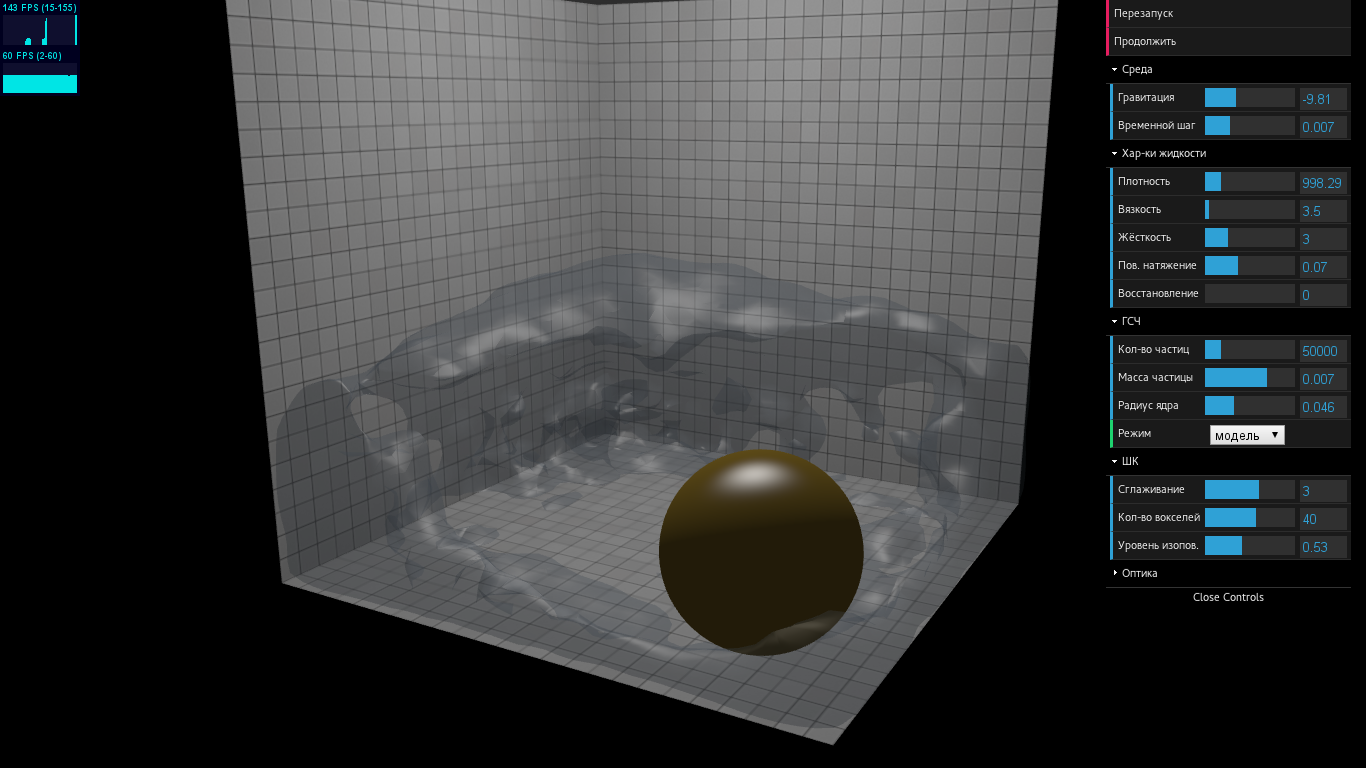
\includegraphics[width=\textwidth]{application.png}
  \caption{Вид приложения.}
  \label{fig:application}
\end{figure}

Для взаимодействия с шаром необходимо нажать на него левой кнопкой мыши и, не отпуская кнопку, передвинуть в нужное место. Для управления камерой необходимо нажать в любое другое место на холсте.
